\chapter{Υλοποιήσεις}
\label{chapter:implementations}

Στο κεφάλαιο αυτό θα αναφερθούμε στο σύστημα που υλοποιήσαμε προκειμένου να πετύχουμε έναν συνδυασμό Ενεργής-Παθητικής Παρακολούθησης με δυνατότητες αυτόματης διευθέτησης πόρων, με σκοπό τη βελτιστοποίηση των υπό μελέτη συστημάτων. Οι βασικές λειτουργίες του συστήματός μας παρατίθενται παρακάτω:\newline

\textbf{Functional Requirements:}
\begin{itemize}
    \item Το σύστημα θα πρέπει να μπορεί να δέχεται URLs καθώς και άλλες πληροφορίες που κρίνονται απαραίτητες για να μπορεί να τα παρακολουθεί, ανά χρονικά διαστήματα που ορίζει ο χρήστης.
    \item Ο χρήστης θα πρέπει να μπορεί να εισάγει κάποια βασικά στοιχεία για τον έλεγχο που θέλει να προσθέσει (url, χρόνο μεταξύ διαδοχικών ελέγχων) καθώς και περαιτέρω στοιχεία που αφορούν το ίδιο το αίτημα που θα πραγματοποιήσει (προσθήκη authorization headers, εκτιμώμενη απάντηση από το σύστημα για validation) 
    \item Το σύστημα θα πρέπει να διαθέτει λειτουργίες scheduler. Να εκτελεί δηλαδή συγκεκριμένες ρουτίνες ανά συγκεκριμένες χρονικές περιόδους.
    \item Το σύστημα θα πρέπει να μπορεί να συλλέγει μεγάλο όγκο δεδομένων και να κρατάει στατιστικά στοιχεία πάνω σε αυτά.
    \item Το σύστημα θα πρέπει να διαθέτει έναν "έξυπνο" μηχανισμό αναγνώρισης ανωμαλιών στους χρόνους αποκρίσεων που συλλέγει κατά τη διάρκεια λειτουργίας του.
    \item Το σύστημα θα πρέπει να μπορεί να συλλέγει δεδομένα κατανάλωσης πόρων από το ίδιο το μηχάνημα που μελετά απομακρυσμένα, εφόσον αυτό έχει μορφή docker container.
    \item Το σύστημα θα πρέπει να μπορεί να τροποποιεί τους διαθέσιμους πόρους του μηχανήματος που ελέγχεται, εφόσον αυτό έχει μορφή docker container.
\end{itemize}

\textbf{Non-Functional Requirements:}
\begin{itemize}
    \item Το scheduling σύστημα θα πρέπει να εκτελεί της ρουτίνες του εντός ορισμένου χρονικού πλαισίου και να μην αποκλίνει από αυτό
    \item Ο αλγόριθμος αναγνώρισης ανωμαλιών θα πρέπει να μην είναι υπολογιστικά "βαρύς", ώστε να εξυπηρετούνται παράλληλα περισσοτεροι από ένας χρήστες
\end{itemize}\mbox{}\\

Γίνεται εμφανές ότι το παραπάνω σύστημα σπάει σε περισσότερα από ένα υποσυστήματα: 

\begin{itemize}
    \item Έναν node express server που στεγάζει το API του συστήματός μας, μοιράζει τις απαραίτητες λειτουργίες στα υπόλοιπα υποσυστήματα και οργανώνει τη ροή της πληροφορίας.
    \item Έναν scheduler, βασική λειτουργία του οποίου είναι να κάνει ping ανά ορισμένα χρονικά διαστήματα URLs (τα οποία είναι αποθηκευμένα σε μία βάση δεδομένων). Πέραν αυτού διαθέτει και άλλες ρουτίνες οι λειτουργίες των οποίων θα αναλυθούν στη συνέχεια.
    \item Αν το υπό μελέτη σύστημα είναι φτιαγμένο με τεχνολογία Docker τότε προστίθεται ένα ακόμα υποσύστημα σε μορφή docker container, που τρέχει στο ίδιο σύστημα με αυτό που μελετάμε και στέλνει logs για την κατανάλωση πόρων των containers που ελέγχουμε. Το υποσύστημα αυτό τροποποιεί δυναμικά τους διαθέσιμους προς τα containers πόρους ανάλογα με τις εντολές που δέχεται απο το σύστημα που θα αναφερθεί στη συνέχεια. Επειδή το υποσύστημα αυτό λειτουργεί σαν μία διάβαση πεζών αυξάνοντας και μειώνοντας τους πόρους προκειμένου να εχουμε λιγότερο συνοστισμό στο εξής θα αναφέρεται ως \textbf{Krosswalk}
    \item Τέλος ένα υποσύστημα που διαβάζει τους χρόνους αποκρίσεων που μαζεύουν οι schedulers κατα τη λειτουργία τους, και κάνει αναγνώριση ανωμαλιών πάνω στα καινούργια δεδομένα που λαμβάνει κάθε φορά. Το υποσύστημα αυτό στέλνει εντολές στο Krosswalk, κάθε φορά που κρίνει ότι υπάρχει κάποια μη φυσιολογική τιμή στη χρονοσειρά που αναλύει. Το σύστημα αυτό στο εξής θα αναφέρεται ως \textbf{Oracle}. 
\end{itemize}

Πλέον και χάριν συντομίας, στο υπόλοιπο κομμάτι της διπλωματικής αυτής εργασίας, θα αναφερόμαστε στο παραπάνω σύστημα, με το όνομα \textbf{Lychte} (/licht/). Η ονομασία αυτή προκύπτει από τα αρχικά του "\textbf{L}ightweight \textbf{Y}et \textbf{C}onfigura\hyp{}ble \textbf{H}ΤTP \textbf{T}raffic \textbf{E}xpert", που περιγράφει την λειτουργία και μερικά μόνο από τα πολλά χαρακτηριστικά του συστήματος μας.

\section{Server}
\label{section:lychte_server}

Αποτελεί τον "εγκέφαλο" του Lychte. Επικοινωνεί άμεσα και έμμεσα με όλα τα υπόλοιπα υποσυστήματα. Οργανώνει τη ροή της πληροφορίας και διαθέτει api μέσω του οποίου μπορούμε να έχουμε πρόσβαση σε όλη την αποθηκευμένη πληροφορία, εφόσον έχουμε τα κατάλληλα κλειδιά authentication και authorization. Πέρα των προαναφερθέντων υποσυστημάτων επικοινωνεί με μία βάση δεδομένων NoSQL και πιο συγκεκριμένα με μια MongoDB.
Η βάση αυτή επιλέχθηκε λόγω της ικανότητάς της να αποθηκεύει μεγάλο όγκο δεδομένων, ο τύπος σχήματος (schema) των οποίων δεν χρειάζεται να είναι αυστηρά προκαθορισμένος. Επιπλέον οι δυνατότητες που παρέχει για sharding καθώς και για εύκολη και γρήγορη κλιμάκωση την καθιστούν ιδανική για το σύστημα μας, που συνεχώς αποθηκεύει νέα δεδομένα στη βάση.

Συνεχίζοντας στο πλαίσιο της βάσης δεδομένων έχουμε ορίσει ορισμένες οντότητες (collections) για την πιο εύκολη αποθήκευση και οργάνωση της πληροφορίας:

\begin{itemize}
    \item \textbf{Api} (\autoref{fig:api_doc}): περιέχει αποθηκευμένες πληροφορίες για τον έλεγχο που θέλουμε να υλοποιήσουμε. Σε αυτές περιλαμβάνονται:
        \begin{itemize}
            \item Μοναδικό ID που περιγράφει μονοσήμαντα το συγκεκριμένο API
            \item Tίτλος
            \item URL
            \item H μέθοδος του url που θέλουμε να ελέγξουμε (GET, POST, PUT, DELETE, PATCH)
            \item O τύπος της αναμενόμενης απάντησης (JSON, STREAM, TEXT)
            \item Ο χρόνος μεταξύ των διαδοχικών ελέγχων
            \item Query παράμετροι που θα στείλουμε μαζί με το url
            \item Body που θα στείλουμε υπό μορφή json στις περιπτώσεις των POST, PUT, DELETE, PATCH αιτημάτων
            \item Headers
            \item Status Code: Το ορίζει ο χρήστης προκειμένου να μπορεί να γίνει έλεγχος αν το αίτημα επιστρέφει αυτό που κανονικά θα έπρεπε
            \item Response body υπό μορφή json: Ομοίως ορίζεται από τον χρήστη για τον λόγο που προαναφέρθηκε 
        \end{itemize}
    \item \textbf{Response} (\autoref{fig:response_docs}): περιέχει αποθηκευμένες πληροφορίες από τα αιτήματα που κάνουμε στα αποθηκευμένα στη βάση apis. Σε αυτά αποθηκεύουμε:
        \begin{itemize}
            \item Το id από το api για το οποίο έχει πραγματοποιηθεί το αίτημα
            \item Ένα πεδίο hasError που περιγράφει το αν το αναμενόμενο (αυτό που έχει ορίσει ο χρήστης) response διαφέρει από το συγκεκριμένο.
            \item Ένα πεδίο hasFailed που δηλώνει σφάλμα κατά την προσπάθεια εκτέλεσης του αιτήματος που οφείλεται σε αποτυχία του Lychte.
            \item Οι χρονισμοί του αιτήματος. Ο χρόνος δηλαδή που χρειάστηκε για να πραγματοποιηθεί το αίτημα, καθώς και όλοι οι χρόνοι στις διάφορες φάσεις εκτέλεσής του (σύνδεση σε DNS server, secure σύνδεση, χρόνος αποστολής πρώτου byte)
            \item Ένα πεδίο που έχει όλη την απάντηση του εξωτερικού συστήματος
            \item Το status code τη στιγμή που πραγματοποιήθηκε το αίτημα
        \end{itemize}
\end{itemize}

\begin{figure}[!ht]
	\centering
	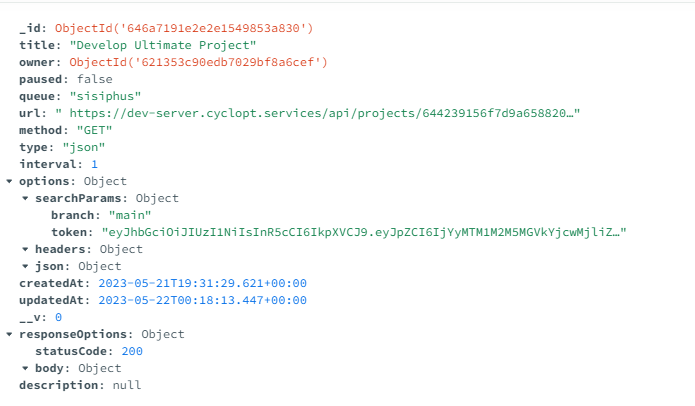
\includegraphics[width=0.9\textwidth]{./images/chapter4/api_doc.png}
	\caption[Παράδειγμα μίας τυπικής εγγραφής API.]{Παράδειγμα μίας τυπικής εγγραφής API.}
	\label{fig:api_doc}
\end{figure}\textbf{}

\begin{figure}[!ht]
	\centering
	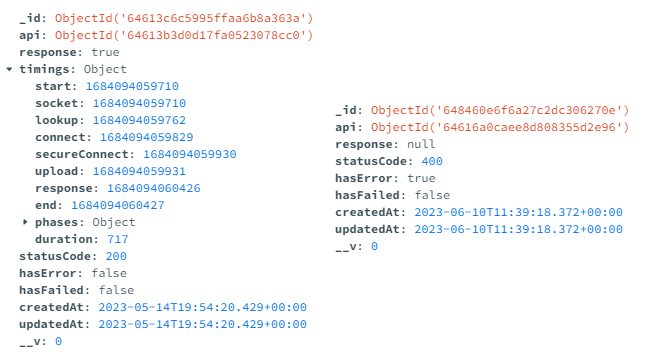
\includegraphics[width=0.9\textwidth]{./images/chapter4/response_docs.png}
	\caption[Παράδειγμα εγγραφών Responses σε αίτημα που πραγματοποιήθηκε επιτυχώς και σε αίτημα που απέτυχε λόγω σφάλματος στο σύστημα που μελετάμε.]{Παράδειγμα εγγραφών Responses σε αίτημα που πραγματοποιήθηκε επιτυχώς και σε αίτημα που απέτυχε λόγω σφάλματος στο σύστημα που μελετάμε.}
	\label{fig:response_docs}
\end{figure}\textbf{}

\section{Scheduler}
\label{section:lychte_scheduler}

Κύρια λειτουργία του συστήματος που υλοποιήσαμε είναι η αυτόματη παρακολούθηση του χρόνου λειτουργίας και απόκρισης ενός ιστότοπου/εφαρμογής. Για να γίνει αυτό θέλουμε ένα υποσύστημα που θα εκτελεί συνέχεια συγκεκριμένα κομμάτια κώδικα σε όσο το δυνατό πιο ακριβής χρονικές στιγμές.

Έχοντας ως ένα κοινό σημείο αναφοράς, τη Mongo βάση, μπορούμε να φτιάξουμε "έξυπνους" schedulers.
Κάθε scheduler θα είναι υπεύθυνος για περισσότερα από ένα apis, στα οποία θα κάνει requests, προκειμένου να δει αν είναι εν λειτουργεία και να ελέγξει την ορθότητα της επιστρεφόμενης απάντησης σε περίπτωση που ο χρήστης έχει ορίσει αναμενόμενη απάντηση. Πλέον και για την πιο οργανωμένη λειτουργία των schedulers προστίθεται ένα ακόμα collection στη βάση. Αυτό ονομάζεται Job (\autoref{fig:sample_job_document} και περιέχει τα εξής πεδία:

\begin{itemize}
    \item Name: η ονομασία του job που εκτελείται. Όπως θα δούμε και στη συνέχεια κάθε scheduler θα έχει παραπάνω από έναν τύπο jobs. Η βασική κατηγορία που θα εμφανίζεται κατά μεγαλύτερο βαθμό είναι η "api" και περιγράφει την εκτέλεση ενός αιτήματος σε ένα url και τον έλεγχο ορθότητάς του.
    \item Data: πληροφορία που είναι αποθηκευμένη στo collection api
    \item repeatInterval: ρυθμός επανάληψης του συγκεκριμένου job (σε ms)
    \item nextRutAt: ο χρόνος σε ms που θα πρέπει να ξανατρέξει το job
    \item lockedAt: πότε ξεκίνησε να εκτελείται (κλείδωσε) το συγκεκριμένο job
    \item Επιπλέον πεδία για την εύκολη αναγνώριση σφαλμάτων (debugging) όπως το (lastFinishedAt, lastRunAt)
\end{itemize}

\begin{figure}[!ht]
	\centering
	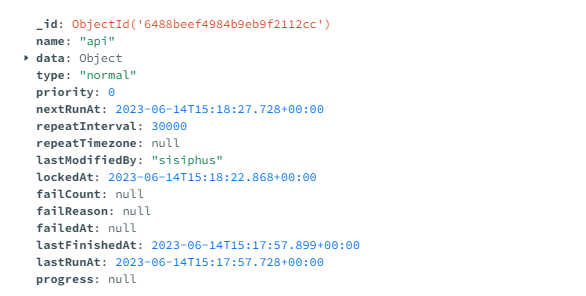
\includegraphics[width=0.8\textwidth]{./images/chapter4/sample_job_document.png}
	\caption[Παράδειγμα εγγραφής ενός \textbf{Job} στη βάση]{Παράδειγμα εγγραφής ενός \textbf{Job} στη βάση. Tο πεδίο \textit{lockedAt} έχει τιμή διάφορη του null, όταν το job ήδη εκτελείται.
		Το πεδίο \textit{nextRunAt} υπολογίζεται από το άθροισμα του χρόνου πλήρωσης της προηγούμενης εκτέλεσής του (\textit{lastFinishedAt}) και του interval. Στο πεδίο \textit{data}
		έχει αποθηκευμένη όλη την πληροφορία που χρειάζεται για να εκτελέσει το αίτημα για το οποίο δημιουργήθηκε το συγκεκριμένο job. Βάσει των πεδίων αυτών κυρίως κρίνεται το αν ο
		κεντρικός scheduler θα ξεκινήσει τη διεργασία}
	\label{fig:sample_job_document}
\end{figure}


Στο πλαίσιο του Lychte μπορούν να υπάρχουν παραπάνω από ένας scheduler που εκτελούν jobs τα οποία ορίζει κάθε φορά ο server. Προκειμένου να έχουμε παραπάνω από έναν scheduler δίνουμε σε κάθε έναν, ένα μοναδικό όνομα. Κάθε scheduler στη συνέχεια πηγαίνει και διαβάζει jobs που είναι αποθηκευμένα στο collection "όνομα-jobs", με αποτέλεσμα να έχεις καταμερισμό των jobs σε περισσότερους από έναν schedulers. Κάθε api πλέον αντιστοιχίζεται μονοσήμαντα σε έναν μόνο scheduler το όνομα του οποίου αποθηκεύεται και στο api που κρατάμε στη βάση κατά τη δημιουργία του. Ο scheduler αποφασίζεται από τον server ανάλογα με το πόσα apis εξυπηρετεί κάθε scheduler εκείνη την χρονική στιγμή.

Η λειτουργία των scheduler περιγράφεται στη συνέχεια. Αρχικά κάθε scheduler ψάχνει κάθε δέκα δευτερόλεπτα στη βάση ποια αιτήματα πρέπει να εκτελεστούν. Πιο συγκεκριμένα ελέγχει ποια jobs στο συγκεκριμένο collection εκτελούνται και πόσα από αυτά θα πρέπει θα πρέπει να εκτελεστούν. Αυτό μπορούμε να το γνωρίζουμε από πριν καθώς κάθε φορά που ξεκινάει ένα job αποθηκεύουμε το χρόνο που ξεκίνησε και υπολογίζουμε το πότε θα πρέπει να ξαναεκτελεστεί (start + repeatInterval). Όλα αυτά γίνονται μόνο εφόσον το job δεν είναι locked (έχει ξεκινήσει αλλά δεν έχει τελειώσει ακόμα). Έτσι αναγνωρίζουμε τις εξής περιπτώσεις χρονισμών:

\begin{itemize}
    \item Επιτυχής Εκτέλεση εντός χρονικού διαστήματος (\autoref{fig:perfect_request_cycle}). Κάθε φορά που έρχεται η στιγμή να ξαναεκτελεστεί το αίτημα έχει ήδη προλάβει να τελειώσει το προηγούμενο
    \item Καθυστερημένη Εκτέλεση αιτήματος (\autoref{fig:timeouts_request_cycle}): Αν κάποιο αίτημα αργήσει να εκτελεστεί, σε χρόνο μεγαλύτερο από το χρόνο που θα πρέπει να ξαναγίνει το αίτημα τότε βάζουμε timeout προκειμένου να λήξουμε πρόωρα το αίτημα και να μην υπάρξουν περαιτέρω καθυστερήσεις στα επόμενα αιτήματα που πρέπει να γίνουν εντός ορισμένου χρονικού διαστήματος
\end{itemize}

\begin{figure}[!ht]
	\centering
	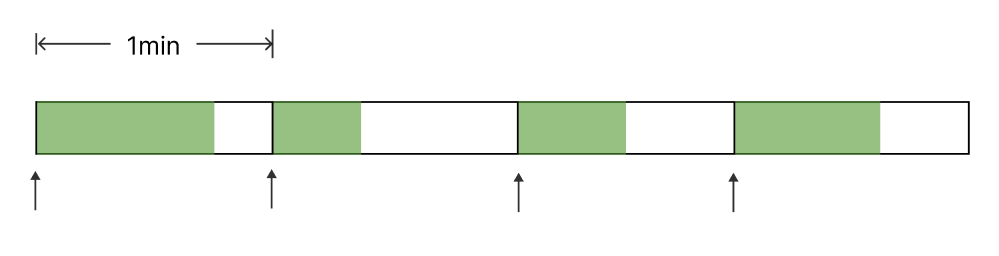
\includegraphics[width=0.8\textwidth]{./images/chapter4/perfect_request_cycle.png}
	\caption[Κύκλος Ζωής εκτέλεσης ενός επαναλαμβανόμενου Αιτήματος με ρυθμό επανάληψης ενός λεπτού]{Κύκλος Ζωής εκτέλεσης ενός επαναλαμβανόμενου Αιτήματος με ρυθμό επανάληψης ενός λεπτού}
	\label{fig:perfect_request_cycle}
\end{figure}

\begin{figure}[!ht]
	\centering
	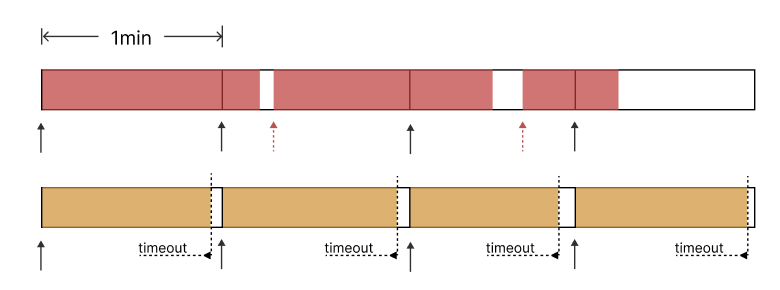
\includegraphics[width=0.8\textwidth]{./images/chapter4/timeout_request_cycle.png}
	\caption[Σύγκριση μη χρήσης και χρήσης timeouts στον κύκλο ζωής εκτέλεσης ενός αργού επαναλαμβανόμενου αιτήματος]{Σύγκριση μη χρήσης ή χρήσης timeouts στον κύκλο ζωής εκτέλεσης ενός αργού επαναλαμβανόμενου αιτήματος. Στην πρώτη περίπτωση το επόμενο αίτημα ξεκινάει μέσα σε χρόνο δέκα δευτερολέπτων από την στιγμή που εκτελέστηκε, με αποτέλεσμα οι χρονισμοί να μην είναι πάντα σταθεροί}
	\label{fig:timeouts_request_cycle}
\end{figure}



% 3.Oracle -> τρέχει τον RePAD2 και αν βρει anomally διαβάζει από το topic "usages" (json της μορφής (cpu: 30\%, ram: 90\% )).Αν κάποιο resource έχει αυξημένη ή μειωμένη χρήση στέλνει στο topic "updates" 

% Όταν κάνεις αναφορά στο oracle αν χρειαστεί να κάνεις επεξήγση του repad βάλε και τα ./images/chapter4/timeseries/repad2/experiment/subplots.png και ./images/chapter4/timeseries/repad2/experiment.png

% \begin{figure}[!ht]
% 	\centering
% 	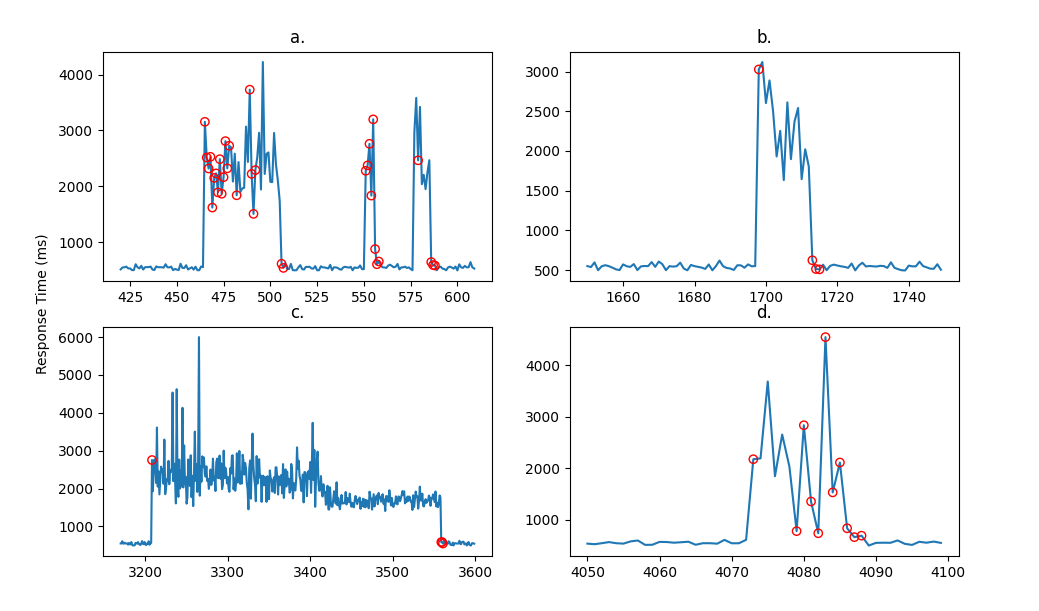
\includegraphics[width=0.9\textwidth]{./images/chapter4/timeseries_repad2_experiment_subplots.png}
% 	\caption[Αποτελέσματα χρήσης της CPU.]{Αποτελέσματα χρήσης της CPU.}
% 	\label{fig:repad2_experiments_subplots}
% \end{figure}

% \begin{figure}[!ht]
% 	\centering
% 	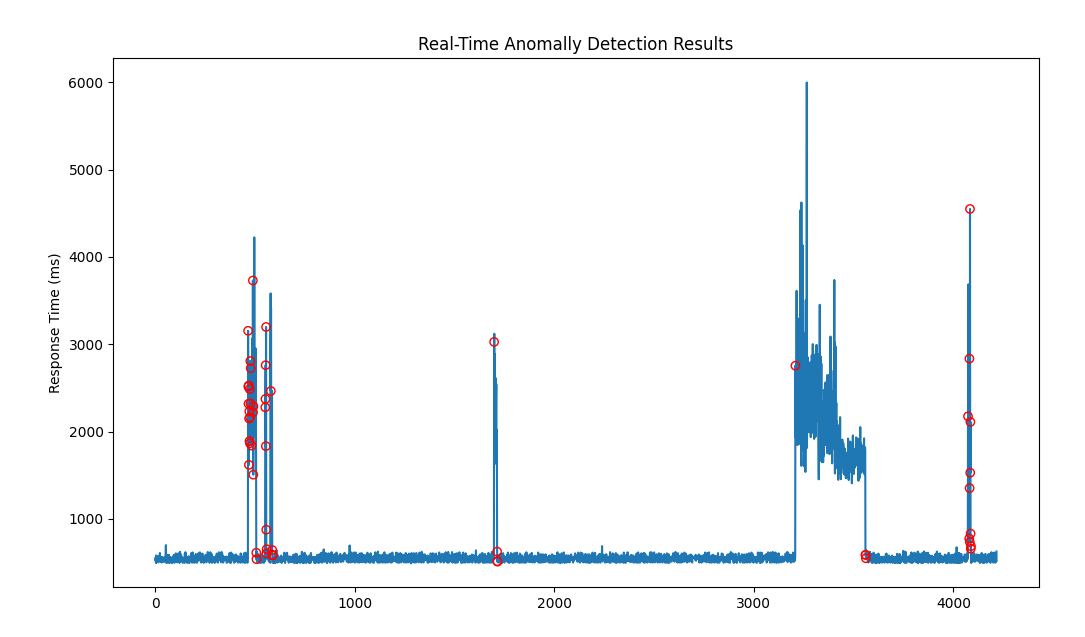
\includegraphics[width=0.9\textwidth]{./images/chapter4/timeseries_repad2_experiment.png}
% 	\caption[Αποτελέσματα χρήσης της CPU.]{Αποτελέσματα χρήσης της CPU.}
% 	\label{fig:repad2_experiments}
% \end{figure}

Όλα αυτά αφορούν αποκλειστικά τη λειτουργία του backend του συστήματος. Πέρα από αυτά
θα πρέπει να υπάρχει μία γραφική διεπαφή, μέσω της οποίας, κάθε χρήστης θα μπορεί να δει τα δεδομένα που παράγονται
από τη χρήση του συστήματός.

Το σύστημα όμως, όπως είναι τώρα, δεν είναι σε θέση να μπορεί να δείχνει επαρκώς γρήγορα ιστορικά δεδομένα. Αν υποθέσουμε ότι έχουμε ένα Api που θέλουμε να ελέγχουμε κάθε
λεπτό, στο τέλος της ημέρας θα έχουν μαζευτεί από αυτό και μόνο 1.440 εγγραφές. Αν αυτά συνεχίζουν να μαζεύονται, τότε ακόμα και τα πιο απλά queries στο μοντέλο των αποκρίσεων θα καθυστερούν, καθιστώντας έτσι την εφαρμογή αργή. Για την αποφυγή συσσώρευσης περιττής, μετά από ορισμένο χρονικό διάστημα, πληροφορίας, έχουμε βάλει επιπρόσθετα σε κάθε scheduler ένα ακόμα job που αφορά
τον καθαρισμό της βάσης από εγγραφές που προέρχονται από το καθένα. Η διεργασία αυτή τρέχει μία φορά την εβδομάδα. Κάθε φορά που εκτελείται ψάχνει τα Apis ανάλογα με τον scheduler στον οποίο τρέχει.
Έπειτα μαζεύει όλες τις αποκρίσεις που σχετίζονται με το κάθε Api ξεχωριστά και ξεκινάει τους υπολογισμούς. Τα δεδομένα που αντλούνται στο πλαίσιο αυτής της διεργασίας, στο τέλος, διαγράφονται από τη βάση, ώστε ολα τα αιτήματα στη βάση να εκτελούνται πιο γρήγορα και αποδοτικά. Σβήνοντας όμως πληροφορία, χάνουμε την ιστορικότητα των δεδομένων μας, με αποτέλεσμα να χάνουν και οι χρήστες μία πιο γενική εικόνα των ελέγχων που έχουν πραγματοποιηθεί. Στο σημείο αυτό εισάγεται μία άλλης μορφής βάση δεδομένων, η Google Cloud Storage.

Πριν σβήσουμε δεδομένα που κρίνουμε ότι δεν είναι απαραίτητο να υπάρχουν στη βάση, αλλά έχουν αξία για ιστορική ανάλυση, τα μεταφέρουμε στο Cloud Storage της Google, υπό μορφή αρχείων.
Με τον τρόπο αυτό κερδίζουμε χώρο, στη κεντρική Mongo βάση, στη λειτουργία της οποίας στηρίζεται όλο το σύστημα, και γενικά απόδοση καθώς έχει καλύτερες ταχύτητες στο σύνολο (\autoref{fig:lychte_server_scheduler}). 

\begin{figure}[!ht]
	\centering
	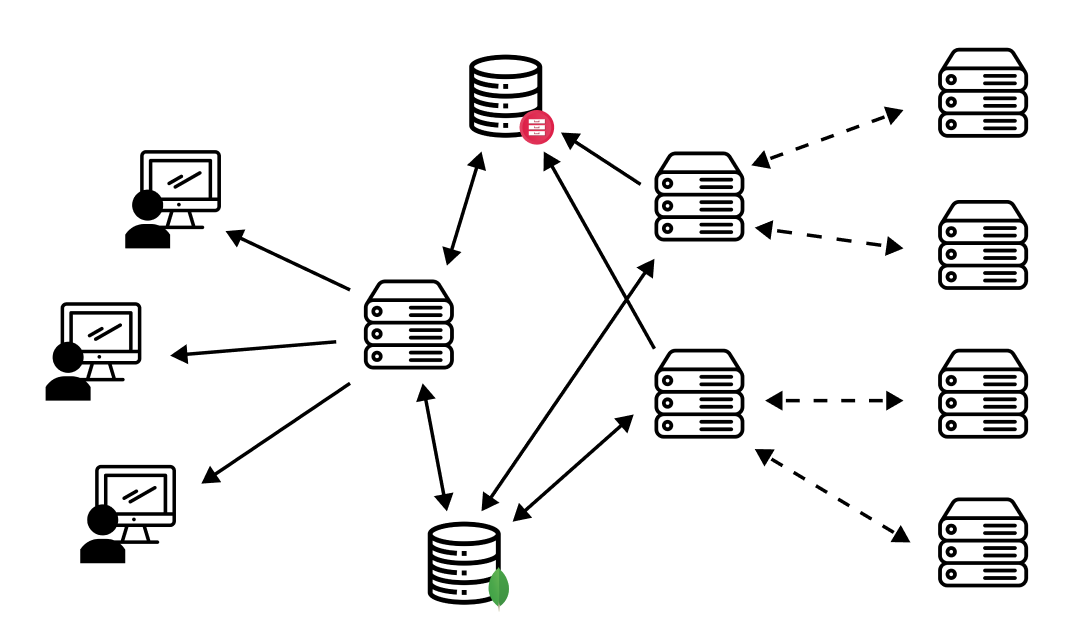
\includegraphics[width=0.8\textwidth]{./images/chapter4/lychte-third-implementation-full.png}
	\caption[Διάγραμμα λειτουργίας Server-Schedulers.]{Διάγραμμα λειτουργίας Server-Schedulers.}
	\label{fig:lychte_server_scheduler}
\end{figure}

Στη συνέχεια θα αναφερθούμε πιο συγκεκριμένα στς βήματα που ακολουθούμε προκειμένου να καθαρίσουμε τη βάση:

\begin{enumerate}
	\item Συλλογή όλων των Responses που υπάρχουν αποθηκευμένα στη βάση, μέχρι μία μέρα πριν την εκτέλεση της διεργασίας καθαρισμού. Αυτό γίνεται προκειμένου να σιγουρευτούμε ότι υπάρχει πάντα πληροφορία στη βάση για την προηγούμενη ημέρα που μπορούμε να δείξουμε.
	\item Δημιουργία δύο διαφορετικών πινάκων, ενός που αποθηκεύει τους χρόνους διάρκειας των αιτημάτων και ενός που περιέχει Boolean μεταβλητές σχετικά με το αν τα αιτήματα γίνονται επιτυχώς ή όχι.
	\item Στη συνέχεια, για κάθε μέρα στην οποία έχουμε εγγραφές Responses, υπολογίζουμε και αποθηκεύουμε στατιστικά σχετικά με τη μέση τιμή, διάμεσο και τυπική απόκλιση διάρκειας των αιτημάτων.
	\item Στο τέλος της διαδικασίας αποθηκεύονται τρία αρχεία για κάθε Api. Ένα στο οποίο περιέχονται τα responses όπως ακριβώς ήταν αποθηκευμένα στη mongodb (σε αρχείο της μορφής \textbf{"../apiId/raw-responses/MM-DD-YYYY.json"}), ένα που περιέχει τους πίνακες που περιγράψαμε στο δεύτερο βήμα (\textbf{"../apiId/\hyp{}raw-values/MM-DD-YYYY.avro"}) και τέλος, ένα αρχείο που περιέχει κάποια χρήσιμα στατιστικά για κάθε μέρα που εντοπίστηκε, όπως περιγράφεται στο βήμα τρία (\textbf{"../apiId/statistics.avro"}) 
\end{enumerate}

Επειδή τα αρχεία που περιέχουν στατιστικά για κάθε μέρα χρησιμοποιούνται αρκετά συχνά από τη γραφική διεπαφή του Lychte για την παρουσίαση ιστορικών δεδομένων του υπό μελέτη Api, κρίναμε απαραίτητη τη χρήση ενός διαφορετικού τύπου αρχείου σε σχέση με
τον κλασσικό και ευρέως διαδεδομένο στο διαδίκτυο τύπο JSON, το AVRO, για να κερδίσουμε ως προς τον αποθηκευτικό χώρο αλλά και την ταχύτητα ανάγνωσης. Αξίζει να σημειωθεί ότι ένα αρχέιο avro σε σχέση με ένα αρχείο json που περιέχουν ακριβώς την ίδια
πληροφορία, για τα στατιστικά στα οποία αναφερόμαστε, είναι 70\% περίπου μικρότερο σε μέγεθος (json αρχείο 250Μb, avro αρχείο 75Μb)
Ο λόγος που μπορούμε να χρησιμοποιήσουμε avro αρχεία είναι ότι η μορφή της αποθηκευμένης πληροφορίας παραμένει ίδια και δεν αλλάζει. Πιο συγκεκριμένα, τα schemas που χρησιμοποιούνται στα αρχεία \textbf{"raw-values/MM-DD-YYYY.avro"} και \textbf{"statistics.avro"}
φαίνονται στο \autoref{fig:avro_types}.

\begin{figure}[!ht]
	\centering
	\makebox[\textwidth][c]{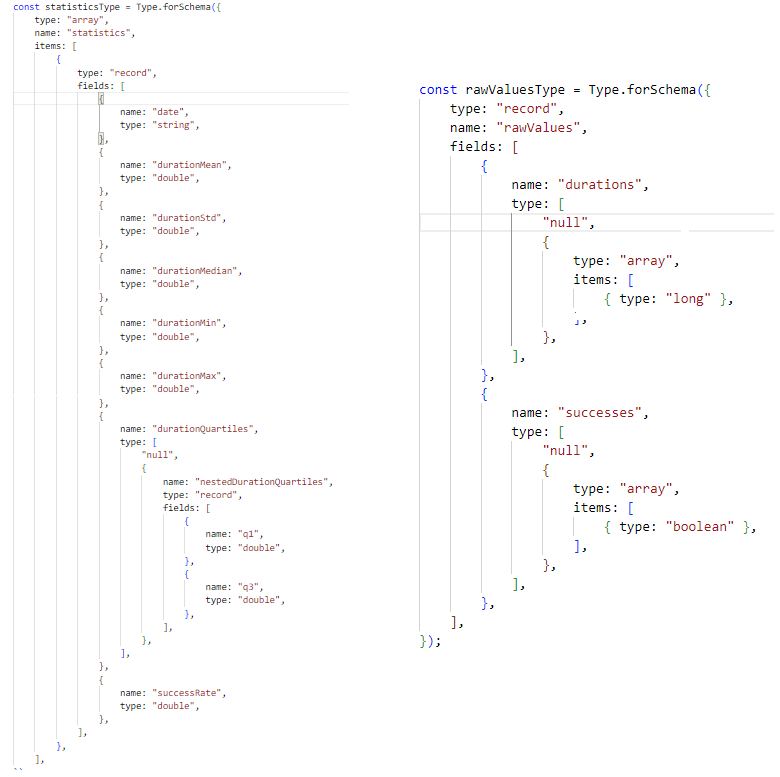
\includegraphics[width=0.87\textwidth]{./images/chapter4/avro_types.png}}
	\caption[Schemas πληροφορίας που αποθηκεύουμε σε avro αρχεία]{Schemas πληροφορίας που αποθηκεύουμε σε avro αρχεία. Το πρώτο αφορά τα statistics που αποθηκεύονται και αποτελείται από ένα array από objects, τα fields των οποίων σχετίζονται σε μετρικές στατιστικής φύσης. Το δεύτερο schema χαρακτηρίζει τα raw-values που αποθηκεύουμε και αποτελείται από ένα object με δύο arrays}
	\label{fig:avro_types}
\end{figure}

\section{Krosswalk}
\label{section:lychte_krosswakl}

Το τρίτο αυτό υποσύστημα μπορεί να υπάρχει εφόσον ο ιστότοπος/εφαρμογή που θέλουμε να ελέγξουμε έχει δημιουργηθεί με εργαλεία docker. Αποτελεί δηλαδή ένα docker container. Το ίδιο έχει πάλι τη μορφή docker container και είναι υπεύθυνο για την συλλογή logs των πόρων του container που θέλουμε να μελετήσουμε και την αποστολή τους σε μία ουρά kafka προκειμένου να έχουμε persistent δεδομένα από τη λειτουργία του. Το krosswalk αποτελεί container που θα πρέπει ο ίδιος ο χρήστης να εγκαταστήσει και να εκτελέσει στο δικό του docker, ώστε να βρίσκεται "δίπλα" σε αυτό που θέλει να ελέγχετε.

Το krosswalk αποτελεί ένα container, που περιέχει ένα εκτελέσιμο αρχείο, το οποίο προήλθε από το "χτίσιμο" κώδικα γραμμένου σε Rust. H γλώσσα πραγραμματισμού Rust επιλέχθηκε κατά κύριο λόγο για την ασφάλεια μνήμης, τις δυνατότητες παράλληλου προγραμματισμού, την αποδοτικότητα που προσφέρει καθώς και τη δυνατότητα δημιουργίας εκτελέσιμων αρχείων (αρχείων που εκτελεί ο υπολογιστής και δεν μπορούν να διαβαστούν από τον άνθρωπο). Αξίζει να σημειωθεί ότι για να κάνουμε έλεγχο ενός συγκεκριμένου container θα πρέπει να γνωρίζουμε το container id του docker container. Αυτό το γνωρίζει μόνο ο χρήστης και το προσθέτει σαν μεταβλητή περιβάλλοντος στο dockerfile του container που περιέχει το krosswalk.

Η βασική λειτουργία του είναι να εκτελεί την εντολή \textit{\textbf{"docker stats cntrId"}} κάθε n (=10) δευτερόλεπτα και να υπολογίζει το ποσοστό χρήσης CPU και RAM του container σε σχέση πάντα με τους διαθέσιμους πόρους που του προσφέρουμε. Αν π.χ. παρέχουμε 0.5cpu και η εκτέλεση της παραπάνω εντολής μας λέει ότι κάνουμε χρήση του 50\% της cpu, τότε καταλαβαίνουμε αμέσως ότι κάνουμε 100\% χρήση της διαθέσιμης cpu, καθώς το docker δίνει το ποσοστό κατανάλωσης όχι ανάλογα με τους διαθέσιμους πόρους αλλά με ποσοστό χρησης της φυσικής cpu του μηχανήματος που τρέχει το container (κάθε 100\% αντιστοιχεί σε 1 physical core). Κάτι παρόμοιο εφαρμόζεται για τον υπολογισμό του ποσοστού χρήσης της μνήμης (RAM). Αυτά στη συνέχεια αποστέλλονται σαν events σε μία ουρά kafka στο topic usages. Εδώ αξίζει να σημειωθεί ότι κάθε φορά που στέλνουμε ένα μήνυμα βάζουμε σαν κλειδί το id του api που αντιστοιχεί στο συγκεκριμένο έλεγχο προκειμένου να μπορούμε να ξεχωρίζουμε ποια usages ανήκουν σε ποια apis. Πέρα από λειτουργίες Kafka Producer θα πρέπει να διαθέτει και λειτουργίες Consumer προκειμένου να τροποποιεί τα resources ανάλογα με τα μηνύματα που θα δέχεται από το επόμενο κατά σειρά υποσύστημα Oracle.

Έτσι στην αρχή λειτουργίας του Krosswalk ξεκινάμε δύο threads, ένα που εκτελεί την παραπάνω διεργασία και ένα που διαβάζει κάθε n (=10) δευτερόλεπτα μηνύματα από τον topic updates, μόνο εφόσον αυτά έχουν σαν κλειδί το id του api που ελέγχουμε. Ανάλογα με το μήνυμα που δέχεται κάθε φορά εκτελεί την εντολή 
\textit{\textbf{"docker update --cpus x --memory y cntrId"}} αυξάνοντας/μειώνοντας τη cpu κατά 0.5 πυρήνες και τη μνήμη κατά 0.5gb. 

\section{Oracle}
\label{section:lychte_oracle}

Αποτελεί το τέταρτο και τελευταίο υποσύστημα του Lychte. Είναι υπεύθυνο για αναγνώριση ανωμαλιών καθώς και την λήψη αποφάσεων σχετικά με το αν θα πρέπει να γίνει αύξηση ή μείωση των διαθεσίμων πόρων, εφόσον έχει εγκατασταθεί το Krosswalk, στο υπό μελέτη σύστημα.

Όπως προαναφέραμε, πριν γίνει οποιαδήποτε τροποποίηση στο σύστημα που μελετάμε κάθε φορά, θα πρέπει πρώτα να βρούμε σημεία στη χρονοσειρά των αποκρίσεων ενός συστήματος που δηλώνουν απόκλιση από το φυσιολογικό. Για να πετύχουμε κάτι τέτοιο χρησιμοποιήσαμε τον αλγόριθμο RePAD2 \cite{lee2023repad2}. Τα βήματα του αλγορίθμου μπορούμε να τα δούμε και στο \autoref{fig:repad2}. Ουσιαστικά εκπαιδεύουμε ένα LSTM με τις τελευταίες τρεις τιμές μάθε φορά της προαναφερθείσας χρονοσειράς και κάνουμε προβλέψεις για την τιμή της τωρινής. Στη συνέχεια υπολογίζουμε ένα δείκτη σφάλματος που συνυπολογίζει τη σχετική διαφορά των τελευταίων τρία κατα σειρά τιμών από τις προβλεπόμενες. Αν αυτό ξεπερνάει ένα threshold (η τιμή του οποίου υπολογίζεται εκ νέου σε κάθε επανάληψη) τότε θεωρούμε ότι υπάρχει εν δυνάμει ανώμαλο σημείο στη χρονοσειρά. Στην περίπτωση που αυτό υπάρξει δημιουργούμε ένα καινούργιο μοντέλο LSTM το οποίο εκπαιδεύεται στα τελευταία τρία σημεία και υπολογίζονται εκ νέου οι μεταβλητές που χρειαζόμαστε (νέα προβλεπόμενη τιμή, νέα τιμή threshold, νέα τιμή σχετικού σφάλματος).

\begin{figure}[!ht]
	\centering
	\makebox[\textwidth][c]{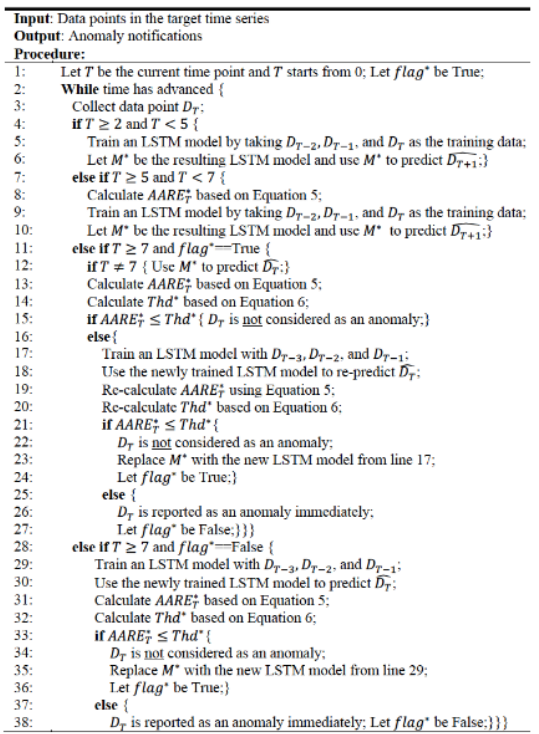
\includegraphics[width=1\textwidth]{./images/chapter4/repad2.png}}
	\caption[Ανάλυση κώδικα REPAD2]{Ανάλυση κώδικα REPAD2}
	\label{fig:repad2}
\end{figure}

Από την παραπάνω λειτουργία παρατηρούμε γρήγορα ότι ένα από τα πλεονεκτήματα του αλγορίθμου είναι το γεγονός ότι δε χρειάζεται μεγάλο αριθμό training data, καθώς για να ξεκινήσει τη λειτουργία του χρειάζεται τρία σημεία κάθε φορά. Στην πραγματικότητα ο εντοπισμός ανώμαλων σημείων γίνεται από τη στιγμή που έχουμε 7 και παραπάνω ενδείξεις καθώς μέχρι το έβδομο σημείο γίνονται οι πρώτοι ακόμα υπολογισμοί των σχετικών σφαλμάτων που θα χρειαστούν σε επόμενα βήματα. Ένα ακόμα πλεονέκτημα είναι ότι τα δεδομένα που του δίνουμε στο στάδιο της εκπαίδευσης δεν έχουν labels. Αναφερόμαστε δηλαδή σε αμιγώς unsupervised learning. Τέλος η «επανεκπαίδευση» δεν γίνεται σε κάθε επανάληψη αλλά μόνο όταν κρίνεται ότι υπάρχει σημείο που αποκλίνει από τη φυσιολογική τάση της χρονοσειράς. Αξίζει να αναφερθεί ότι η διαδικασία δημιουργίας καινούργιου LSTM ειναι πολύ γρήγορη (0.2 δευτερόλεπτα κατά μέσο όρο) με αποτέλεσμα οι προβλέψεις που κάνουμε να πλησιάζουν συμπεριφορά real time (ακόμα και στην περίπτωση που πρέπει να ξαναφτιάξουμε καινούργιο μοντέλο).

Ο παραπάνω αλγόριθμος, στο πλαίσιο αυτής της διπλωματικής αναφοράς, υλοποιήθηκε με χρήση της προγραμματιστικής γλώσσας python και κατά κύριο λόγω με βιβλιοθήκες αυτής όπως οι pandas και numpy για την αποθήκευση/τροποποίηση δεδομένων και η tensorflow για τη δημιουργία, διαχείρηση, αποθήκευση machine learning μοντέλων. Η αποθήκευση των δεδομένων που χρειάζονται σε μελλοντικά στάδια του αλγορίθμου όπως είναι ο δείκτης σχετικού σφάλματος και οι προβλέψεις που κάνουμε σε κάθε βήμα αποθηκεύονται στη βάση mongo, στο αντίστοιχο collection responses κάθε φορά, τροποποιώντας έτσι ελάχιστα το schema που είχαμε ορίσει στην αρχή του κεφαλαίου. Το python script έχει έναν mini scheduler που ξεκινάει τον επαναληπτικό αλγόριθμο. Αυτός καλείτε κάθε m (=10 δευτερόλεπτα) για κάθε api που θέλουμε να κάνουμε real time anomaly detection).

Αφού γίνει η αναγνώριση «σφάλματος» στο υπό μελέτη σύστημα θα πρέπει να γίνεται και διόρθωση αυτού. Σε αυτό το σημείο έρχεται το Krosswalk και η Kafka ουρά στην οποία κρατάμε δεδομένα για τη λειτουργία του συστήματος (εφόσον όπως έχουμε ήδη αναφέρει αποτελεί docker container και έχει εγκατασταθεί το Krosswalk σε ένα container εντός του υπό μελέτη συστήματος). Συνεπώς μετά την αναγνώριση λάθους το python script ξεκινάει να λειτουργεί σαν Kafka Consumer. Διαβάζει events από το topic usages μέχρι να βρει κάποιο που προέρχεται από το api που αναλύει εκείνη τη στιγμή. Αν εντός k δευτερολέπτων δε λάβει απάντηση συνεχίζει κανονικά τη λειτουργία του σε μια επόμενη επανάληψη. Αν λάβει κάποιο μήνυμα τότε ανάλογα με το ποσοστό χρήσης της μνήμης και της CPU στέλνει ανάλογα μηνύματα για την αύξηση ή μείωση του καθενός ξεχωριστά. Πιο συγκεκριμένα αν το ποσοστό χρήσης ξεπερνά το 90\% τότε αυξάνει τους πόρους και αν είναι κάτω του 10\%, τους μειώνει κατά μια μονάδα κάθε φορά (0.5 πυρήνες για τη cpu και 0.5gb για τη μνήμη). Για να μεταφερθεί η πληροφορία τροποποίησης των πόρων στο Krosswalk, το Oracle στέλνει ένα event στο topic updates με συγκεκριμένες κάθε φορά εντολές.

Προκειμένου να δούμε καλύτερα τη λειτουργία του αλγορίθμου RePAD2 και να μελετήσουμε την αποτελεσματικότητα του στο δικό μας σύστημα έχουμε πάρει πραγματικά δεδομένα απο χρονικές αποκρίσεις ενός συστήματος και τον εφαρμόσαμε πάνω σε αυτά. Οι αποκρίσεις φαίνονται στο \autoref{fig:repad2_experiments}. Με κόκκινα κυκλάκια σηματοδοτούμε τα σημεία στα οποία η εφαρμογή του αλγορίθμου εντοπίζει ανώμαλα σημεία. Για να γίνουν πιο εμφανή τα σημεία που εντοπίστηκαν, στο \autoref{fig:repad2_experiments_subplots} μπορούμε να τα δούμε σε μεγέθυνση. Αξίζει να σημειωθεί ότι και στις έξι περιπτώσεις που έχουμε ανώμαλα σημεία, τέτοια δηλαδή που αποκλίνουν από τους φυσιολογικούς χρονισμούς που παρατηρούνται, ο εντοπισμός γίνεται τόσο στην αρχή της αύξησης του φόρτου του υπο μελέτη συστήματος όσο και στη μείωση αυτού. Στις πρώτες τρεις μάλιστα περιπτώσεις αύξησης του φορτίου βλέπουμε ότι παρατηρούνται περισσότερα από ένα συνεχόμενα σημεία που αναγνωρίζονται ως ανώμαλα. Κάτι το οποίο σε επόμενες περιπτώσεις δε συμβαίνει αφού ο εντοπισμός γίνεται στην αρχή και στο τέλος της τροποποίησης του φορτίου. Αυτό γίνεται διότι ο τρόπος που υπολογίζεται το όριο απόφασης (decision threshold) εμπεριέχει όλες τις προηγούμενες τιμές σχετικού λάθους. Με αποτέλεσμα όσο περισσότερα δεδομένα υπάρχουν τόσο πιο ανθεκτικός να είναι σε μικρότερες μεταβολές.

\begin{figure}
    \centering
	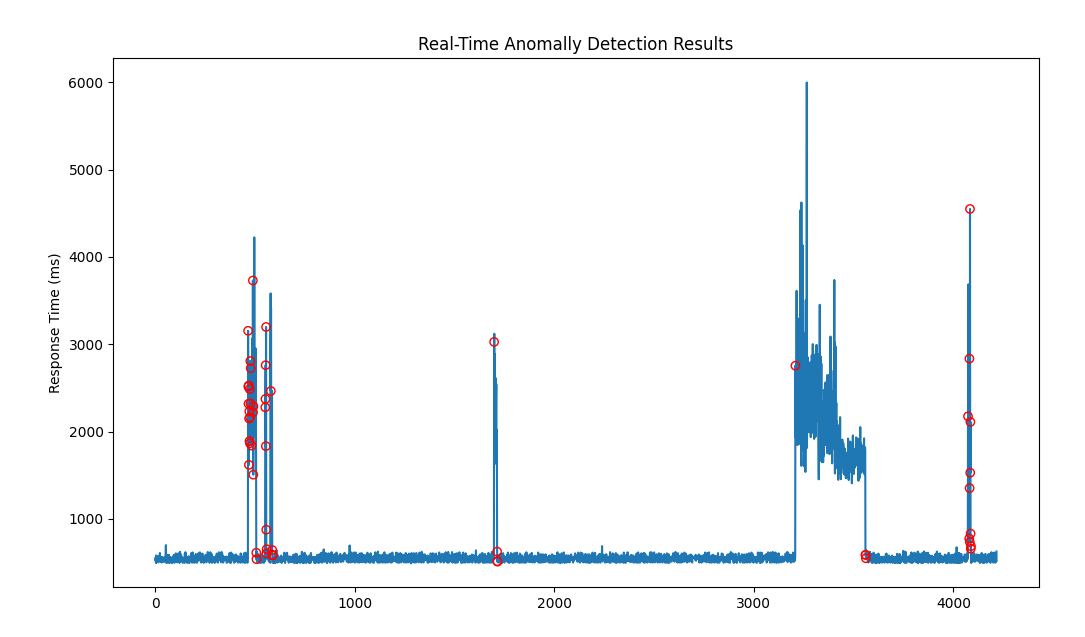
\includegraphics[width=0.9\textwidth]{./images/chapter4/timeseries_repad2_experiment.png}
	\caption[Χρονοσειρά αποκρίσεων ενός συστήματος που προήλθε απο τη χρήση του συστήματος Lychte. Με κόκκινο φαίνονται τα ανώμαλα σημεία που εντοπίστηκαν απο τη χρήση του RePAD2.]{Χρονοσειρά αποκρίσεων ενός συστήματος που προήλθε απο τη χρήση του συστήματος Lychte. Με κόκκινο φαίνονται τα ανώμαλα σημεία που εντοπίστηκαν απο τη χρήση του RePAD2.}
	\label{fig:repad2_experiments}
\end{figure}

\begin{figure}
	\centering
	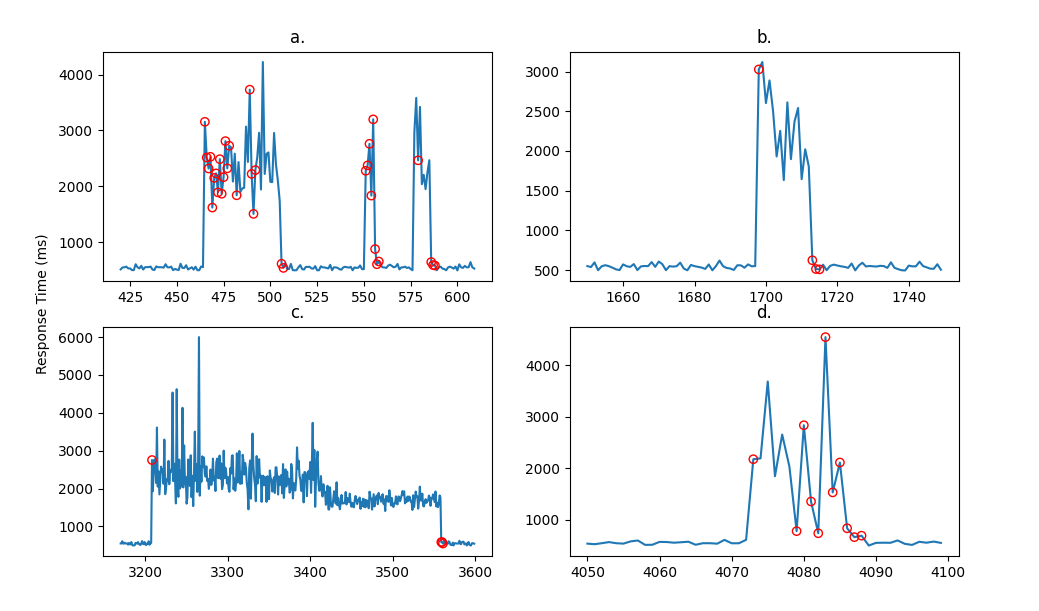
\includegraphics[width=0.9\textwidth]{./images/chapter4/timeseries_repad2_experiment_subplots.png}
	\caption[Εντοπισμένα σημεία ανωμαλιών σε μεγέθυνση.]{Εντοπισμένα σημεία ανωμαλιών σε μεγέθυνση.}
	\label{fig:repad2_experiments_subplots}
\end{figure}
